\chapter{Inverse Solutions}
\label{ch:inv}

\section{Overview}

The inverse problem of electrocardiography is to find suitable electrical source parameters on the heart that adequately describe the observed body surface potentials. Regularization is typically employed in solution methods to reduce the sensitivity of the problem to relatively small errors in the observed body surface potentials, thereby stabilizing it. As a result, solution methods may be supplied body surface potentials, a forward model, and method-specific regularization parameters as input. Specific use of each method is described below. As output, modules primarily produce the resulting solution with extra outputs depending on the specific method.

\section{Module Descriptions for Inverse Solution Methods}

%%%%%%%%%%%%%%%%%%%%%%%
\subsection{Tikhonov Regularization}

\begin{figure}[H]
\begin{center}
\includegraphics[width=\textwidth]{ECGToolkitGuide_figures/SolveInverseProblemWithTikhonov.png}
\caption{Tikhonov Regularization Module}
\label{tikhonov}
\end{center}
\end{figure}

\vspace{5pt}\textit{This is a method of solving the potential-based inverse problem.}\vspace{5pt}

Tikhonov regularization is a common method of stabilizing solutions to many inverse problems including inverse ECG. The module that implements Tikhonov regularization (closed-form solution) in SCIRun is called ``SolveInverseProblemWithTikhonov''. The module requires that a forward solution matrix, regularization matrix (such as a surface Laplacian approximation), and a vector (single-column matrix) of observed/measured body surface potentials are supplied as input.

In the user interface (UI), one can explicitly specify a scalar regularization parameter that weights the influence of the regularization matrix on the solution. The module can also automatically select a regularization parameter using the L-curve method.

Upon completion, the module will output the inverse solution. In addition, it will either output the specified or automatically-chosen regularization parameter as well as the regularized inverse matrix (a closed-form Tikhonov inverse operator).


%%%%%%%%%%%%%%%%%%%%%%%
\subsection{Tikhonov Singular Value Decomposition (SVD)}

\begin{figure}[H]
\begin{center}
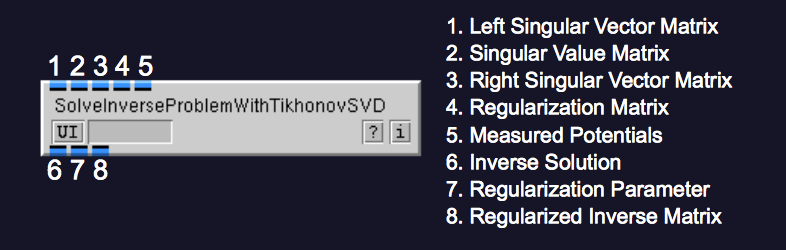
\includegraphics[width=\textwidth]{ECGToolkitGuide_figures/SolveInverseProblemWithTikhonovSVD.png}
\caption{Tikhonov SVD Module}
\label{tikhonovsvd}
\end{center}
\end{figure}

\vspace{5pt}\textit{This is a method of solving the potential-based inverse problem.}\vspace{5pt}

This module implements Tikhonov regularization (closed-form solution) using the singular value decomposition (SVD) in SCIRun and is called ``SolveInverseProblemWithTikhonovSVD''. The module requires that the SVD of a forward solution matrix (left/right singular vector matrices and singular value matrix), regularization matrix (such as a surface Laplacian approximation), and a vector (single-column matrix) of observed/measured body surface potentials are supplied as input.

In the user interface (UI), one can explicitly specify a scalar regularization parameter that weights the influence of the regularization matrix on the solution. The module can also automatically select a regularization parameter using the L-curve method.

Upon completion, the module will output the inverse solution. In addition, it will either output the specified or automatically-chosen regularization parameter as well as the regularized inverse matrix (a closed-form Tikhonov inverse operator computed using the provided SVD).

%%%%%%%%%%%%%%%%%%%%%%%
\subsection{Truncated SVD}

\begin{figure}[H]
\begin{center}
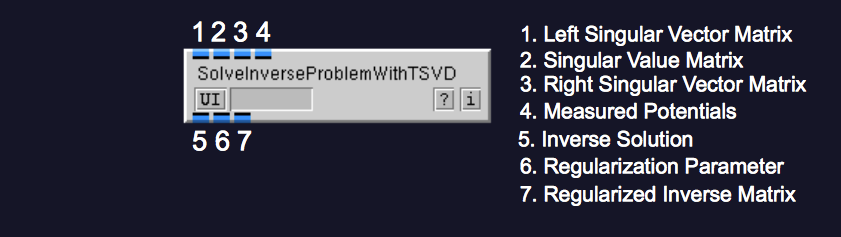
\includegraphics[width=\textwidth]{ECGToolkitGuide_figures/SolveInverseProblemWithTSVD.png}
\caption{Truncated SVD Module}
\label{tsvd}
\end{center}
\end{figure}

\vspace{5pt}\textit{This is a method of solving the potential-based inverse problem.}\vspace{5pt}

This module, called ``SolveInverseProblemWithTSV'', computes an inverse solution by creating a pseudo-inverse operator and multiplying that with the measured body surface potentials. The module requires that the SVD of a forward solution matrix (left/right singular vector matrices and singular value matrix) and a vector of observed/measured body surface potentials are supplied as input.

In the user interface (UI), one can explicitly specify a scalar integer regularization parameter to control the amount of regularization imposed on the problem. Assuming the singular values are sorted from largest to smallest (and therefore most significant to least significant), the regularization parameter controls how many significant singular values to consider (truncation degree) when calculating the pseudo-inverse. Alternatively, the module will use the L-curve method to automatically obtain a suitable truncation degree.

The primary output of this module is a vector containing the inverse solution. In addition, it will output the regularization parameter and regularized inverse operator used to obtain the inverse solution from the measured body surface potentials.

%%%%%%%%%%%%%%%%%%%%%%%%%

\subsection{Matlab Interface}

The \textit{InterfaceWithMatlab} module allows a SCIRun network to make use of Matlab for some of its calculations. In Figure \ref{matlabinterfacemodule}, the user interface for this module shows how SCIRun data types from the module's input pipes are converted to Matlab variables for use in a Matlab script. Upon completion of the Matlab script, Matlab variables are converted back to SCIRun data types to be sent to the module's output pipes.

\begin{figure}[H]
\begin{center}
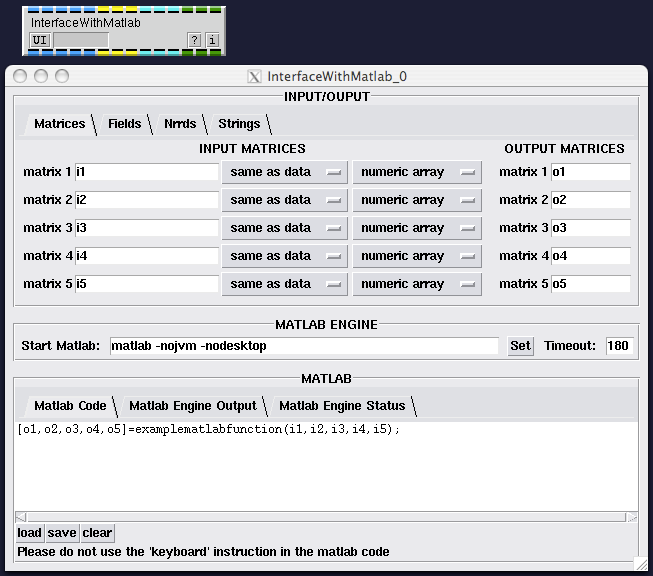
\includegraphics[width=0.8\textwidth]{ECGToolkitGuide_figures/InterfaceWithMatlab.png}
\caption{The InterfaceWithMatlab Module and its corresponding user interface}
\label{matlabinterfacemodule}
\end{center}
\end{figure}

In the rest of this section, we will describe some of the inverse solution methods distributed with SCIRun that have been implemented in Matlab.


\subsubsection{Isotropy Method}

\vspace{5pt}\textit{This is a method of solving the potential-based inverse problem.}\vspace{5pt}

\begin{verbatim}
function X_reg=greensite(A,Y,trunc_deg)
% Function to calculate the Greensite inverse solution
%   A - forward matrix
%   Y - data
%   trunc_deg - truncation degree
%   X_reg - inverse solution
\end{verbatim}

The isotropy method (a.k.a. Greensite method) takes as input a forward solution matrix, measured body surface potential data, and an optional integer regularization parameter (truncation degree). In this method, the truncation degree controls the number of significant singular values of the measured body surface potential data to be used when computing the inverse solution. Consequently, the truncation degree partitions the measured body surface potential data into independent ``signal'' and ``noise'' components, ignoring the ``noise'' component in its calculation of the inverse solution. The only output of the method is the inverse solution.

\subsubsection{Gauss-Newton Method}

\vspace{5pt}\textit{This is a method of solving the activation-based inverse problem.}\vspace{5pt}

\begin{verbatim}
function tau = ActGaussNewton(A,Y,L,tauinit,lambda,w,minstep)
% Implements the Gauss-Newton algorithm for solving the activation-based
% inverse problem of electrocardiography.
% => minimizes the objective function ||Y-A*X||^2+lambda*||L*X||^2 where
% X is parameterized by the C^1 polynomial approximation to a step function
% as explained in "The Depolarization Sequence of the Human Heart Surface
% Computed from Measured Body Surface Potentials" by Geertjan Huiskamp and
% Adriaan van Oosterom.
% 
% Input Variables:
% A: Forward matrix
% Y: Observations (columns index time from 1 to T=size(Y,2))
% L: Regularization matrix (typically a surface Laplacian approximation)
% lambda: Regularization parameter
% w: Width parameter in step function approximation
% tauinit: Initial phase shifts for starting the algorithm
% 
% Output Variables:
% tau: Solution phase shifts of the step functions
\end{verbatim}

The activation-based inverse problem of electrocardiography is to solve for electrical activation times (i.e. depolarization times) on the heart given body surface potentials during the QRS complex. This results in a nonlinear least squares optimization problem that this method solves using the Gauss-Newton algorithm. Solutions are typically highly dependent on choice of initial guess. This method requires a forward solution matrix, body surface potentials, regularization matrix, initial guess, regularization parameter, activation waveform transition width, and convergence parameter to be specified as input. The body surface potentials should be provided as a $M \times T$ matrix, where $M$ is the number of leads from which potentials are recorded and $T$ is the number of time samples recorded during the QRS complex of the heart beat whose activation times are to be estimated. The regularization matrix and corresponding parameter influence the inverse solution as in Tikhonov regularization (see above). The initial guess is the set of activation times from which the Gauss-Newton algorithm starts pursuing a more suitable inverse solution. The transition width controls the number of time samples (not necessarily integer) taken by each source to transition from inactivated to activated in this method. The convergence parameter is the minimum norm of the step taken by the iterations within the Gauss-Newton algorithm before the method is deemed to have converged to a suitable solution. The only output of the method is the inverse solution (in this case: an array/vector of activation times).

\subsubsection{Wavefront-Based Potential Reconstruction}

\vspace{5pt}\textit{This is a method of solving the potential-based inverse problem.}\vspace{5pt}

\begin{verbatim}
function [x_WBPR_forward,x_WBPR_backward] = WBPR(A,y,heart,first_act,last_act)
% Function to calculate the WBPR solutions
% Inputs:
%   A: forward matrix
%   y: torso data
%   heart: heart geometry
%   first_act: first activated node
%   last_act: last activated node
%
% Outputs:
%   x_WBPR_forward: inverse solution using forward WBPR
%   x_WBPR_backward: inverse solution using backward WBPR
\end{verbatim}

The Wavefront-Based Potential Reconstruction (WBPR) method imposes prior knowledge about the spatial patterns of electric potentials on the heart during the QRS complex to reconstruct an inverse solution. This method requires a forward solution matrix, measured body surface potentials, a structure containing the triangles and nodes of the heart geometry mesh, and the first/last nodes to activate during the QRS complex of the heart beat. The body surface potentials should be provided as a $M \times T$ matrix, where $M$ is the number of leads from which potentials are recorded and $T$ is the number of time samples recorded during the QRS complex of the heart beat whose electric potentials are to be estimated. The heart geometry is a Matlab ``struct'' that must contain a matrix of node coordinates and a matrix of indices for triangles that connect the nodes on the surface of the heart. The first/last nodes to activate are specified as the indices of the nodes.

As output, WBPR produces two inverse solutions. The procedure by which the inverse solutions are obtained may be run both forward and backward in time. Therefore, the ``forward WBPR'' solution is that obtained by applying the method starting from the earliest sample time and ending at the latest. On the other hand, the ``backward WBPR'' solution is obtained by starting from the latest sample time and traversing the samples in reverse until ending at the earliest.

%%%%%%%%%%%%%%%%%%%%%%%%%

\section{Example Simulations}

\subsection{Tikhonov Regularization}

\vspace{5pt}\textit{The SCIRun network for this example can be found at:\\``\{ECGTOOLKITDIRECTORY\}/potential-based-inverse/tikhonov-inversion.srn''\\in the SCIRun source code directory.}\vspace{5pt}

\begin{figure}[H]
\begin{center}
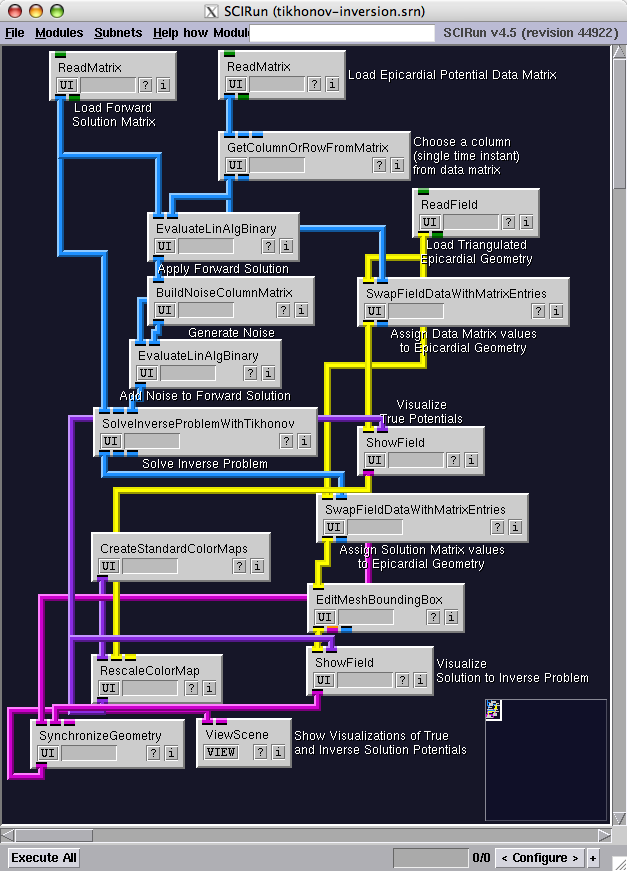
\includegraphics[width=0.9\textwidth]{ECGToolkitGuide_figures/TikhonovNetwork.png}
\caption{The SCIRun network for the Tikhonov inverse solution example.}
\label{TikhonovNetworkExample}
\end{center}
\end{figure}

This example shows how to use the ``SolveInverseProblemWithTikhonov'' module in a SCIRun network to solve a potential-based ECG inverse problem using Tikhonov regularization. Specifically, this example simulates ``measured'' body surface potentials by applying a forward solution and adding pseudorandom noise with a specified signal-to-noise ratio (SNR). The forward solution is obtained by multiplying a known vector of epicardial potential data by a pre-computed forward solution matrix. The simulated measurements and forward solution matrix are the inputs to the ``SolveInverseProblemWithTikhonov'' module. The regularization parameter of this method is controlled via the user interface (UI) in this example. The output from the module is the inverse solution. This example compares the inverse solution to the known epicardial potentials from which the measurements were simulated. A visualization of both can be seen in the UI of the ``ViewScene'' module.

\subsection{Gauss-Newton Method}

\vspace{5pt}\textit{The SCIRun network for this example can be found at:\\``\{ECGTOOLKITDIRECTORY\}/activation-based-inverse/actgaussnewton-inversion.srn''\\in the SCIRun source code directory.}\vspace{5pt}

\begin{figure}[H]
\begin{center}
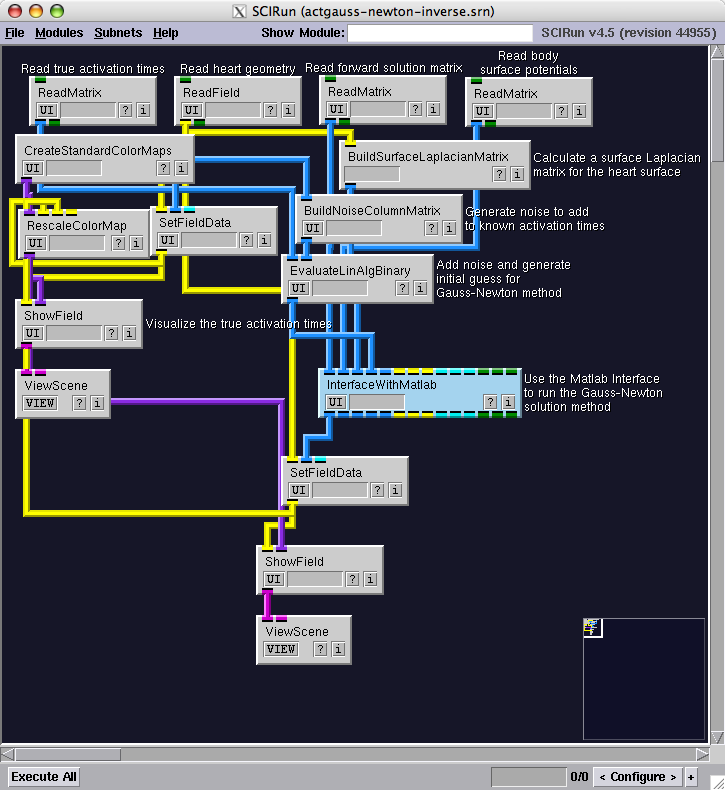
\includegraphics[width=0.9\textwidth]{ECGToolkitGuide_figures/actgaussnewtonnetwork.png}
\caption{The SCIRun network for the activation-based Gauss-Newton inverse solution example.}
\label{GaussNewtonNetworkExample}
\end{center}
\end{figure}

This example shows how to use the ``InterfaceWithMatlab'' module in a SCIRun network to solve an activation-based ECG inverse problem using the Gauss-Newton method. This example uses the ``normal male'' dataset and geometries from ECGSIM. Specifically, this method compares measured body surface potentials with body surface potentials simulated from activation times. We search the set of possible activation times for ones that minimize the squared error residual between the measured and simulated body surface potentials. The Gauss-Newton method in this example is implemented as a Matlab function and is used in SCIRun via the ``InterfaceWithMatlab'' module. As a numerical optimization method, Gauss-Newton will look for a local minimizer of the squared error residual starting from a suitable initialization point. In this example, we initialize the method with the activation times reported for the dataset in ECGSIM, but perturbed by noise.

